\section{Summaries}
\subsection{COOP – Strategies for Sustainable Food}

Coop is one of the largest retailers in Switzerland. Coop can look back on a History spanning over 150 years. Coop is still a cooperative because some several advantages, for example: for sustainability and long-term thinking. The Strategic concept for sustainability by Coop stand on three columns, which are:\\

-Sustainable assortment performance\\
-Resource efficiency and climate protection\\
-Employees and society\\

All these points are equally important for a company that wants to act sustainably.
In the long history of Coop, they had some milestones about sustainability. For example in 1993, Coop launched Naturaplan, Naturaline and Max Havelaar. 
The Max Havelaar foundation, which is the most famous of Coops launched foundations, is a NGO, which stand for fair-trade, and awards the fair-trade label for sustainable and fair-trade products. The benefits of this organisation is to improve the livelihood of the developing world. You can find these labels on different products such as honey, coffee, tea, bananas, cacao, cotton, pineapples, flowers, mango, orange juice, rice and sugar.
In addition, a big point in the sustainable food strategies by Coop is the thematic about the palm oil. Many areas, which are now palm oil farms, were once rainforests. So many farmers used to burn the rainforest down to increase the amount of the palm oil. Coop is very focused on selling only products from sustainable palm oil cultivation. On this point Coop is working together with the WWF to get on this goal.
For Coop Sustainable palm oil means:
– No uprooting of virgin forests and valuable living space
– Protection of water, soil, air, animals and plants
– Compliance with land use‐ and proprietary‐rights
– No child work, involving small farmers.

Coop is not only trying to sell sustainable products but also to be sustainable. For example, they want to be CO2 Neutral by the year 2023. 
In order to achieve this goal, those used, for example, to transport the goods trucks, which are driven with hydrogen instead of using conventional fuel. 

From 2003 on, they spend each year 10 Million Swiss Francs into the Foundation of Coop Naturaplan‐fund. In addition Coop spend also 16,6 Million Swiss Francs in about 70 projects which have different goals such as innovations, Raising awareness of broad public by broad communication concerning sustainability and also Compensation of CO2‐emissions.

Coop is also committed to sustainability in the social field. This is done for different reasons. One part of the unsold food will be donated to the {}\grqq Swiss table{}\grqq and {}\grqq Tischlein deck dich{}\grqq . Another aspect is that Coop also draws attention to sustainable products, and not least by labels, which have been launched by their own. As mentioned earlier in the text, Coop has launched some own labels.  For Coop, it is also a big concern to be able to infomate its customers and lables are there a good way.

Overall, Coop is a company that is very concerned about sustainability and has been around for a long time. Coop also has ambitious future plans and sustainability is also being improved in various areas.
\subsection{Options
	for
	Change
	– Innovation
	in
	Food
	Affair}

The consumer has in fact a lot of power. No company produces something, nobody buys.  Instead of
forcing companies to produce sustainably it's more effective and, yes, sustainable to change the
customer's behaviour.  The problem is, the power is distributed over a lot of people. Therefore you
have to convince people to change.

Most decisions in a daily life are decided automatically, without a proper evaluation. That's
because we can  rely on the experience of former decisions and link compareable knowledge to current
situations. We only take new information into account which is presented to us in the very moment of
the decision.

So there is an opportunity to nudge the consumer in the desired direction. You can show the consumer
the effects of his decision right before he decides.

The nudge is only effective if the consumer is both aware of his behaviour and willing and able to
change. If he is only willing and able to change but lacks awareness there has to be education.

If the consumer is aware of the problem but cannot afford a change, you can help him by putting an
incentive.

If he lacks both awareness and willingness, a big effort has to be made to change this fella's
behaviour.

Often there is a default option. Most poeple rely on this option too. So if you change this it
has a huge impact on consumer behaviour.

\newpage

\subsection{Sustainable Development
	and Food Security}
The World Commission on Environment published in 1987 a new concept - sustainable development. It became one of the most successful concept introduce in many years. They defined sustainable as "development which meets the needs of current generations without compromising the ability of future generations to meet their own needs" \cite{_our}it also underlines the importance of protecting the natural resource base and the environment. They defined 17 main Goal Each goal has specific targets to be achieved over the next 15 years. For the goals to be reached, everyone needs to work together to reach them.

\begin{figure}[H]	
	\centering
	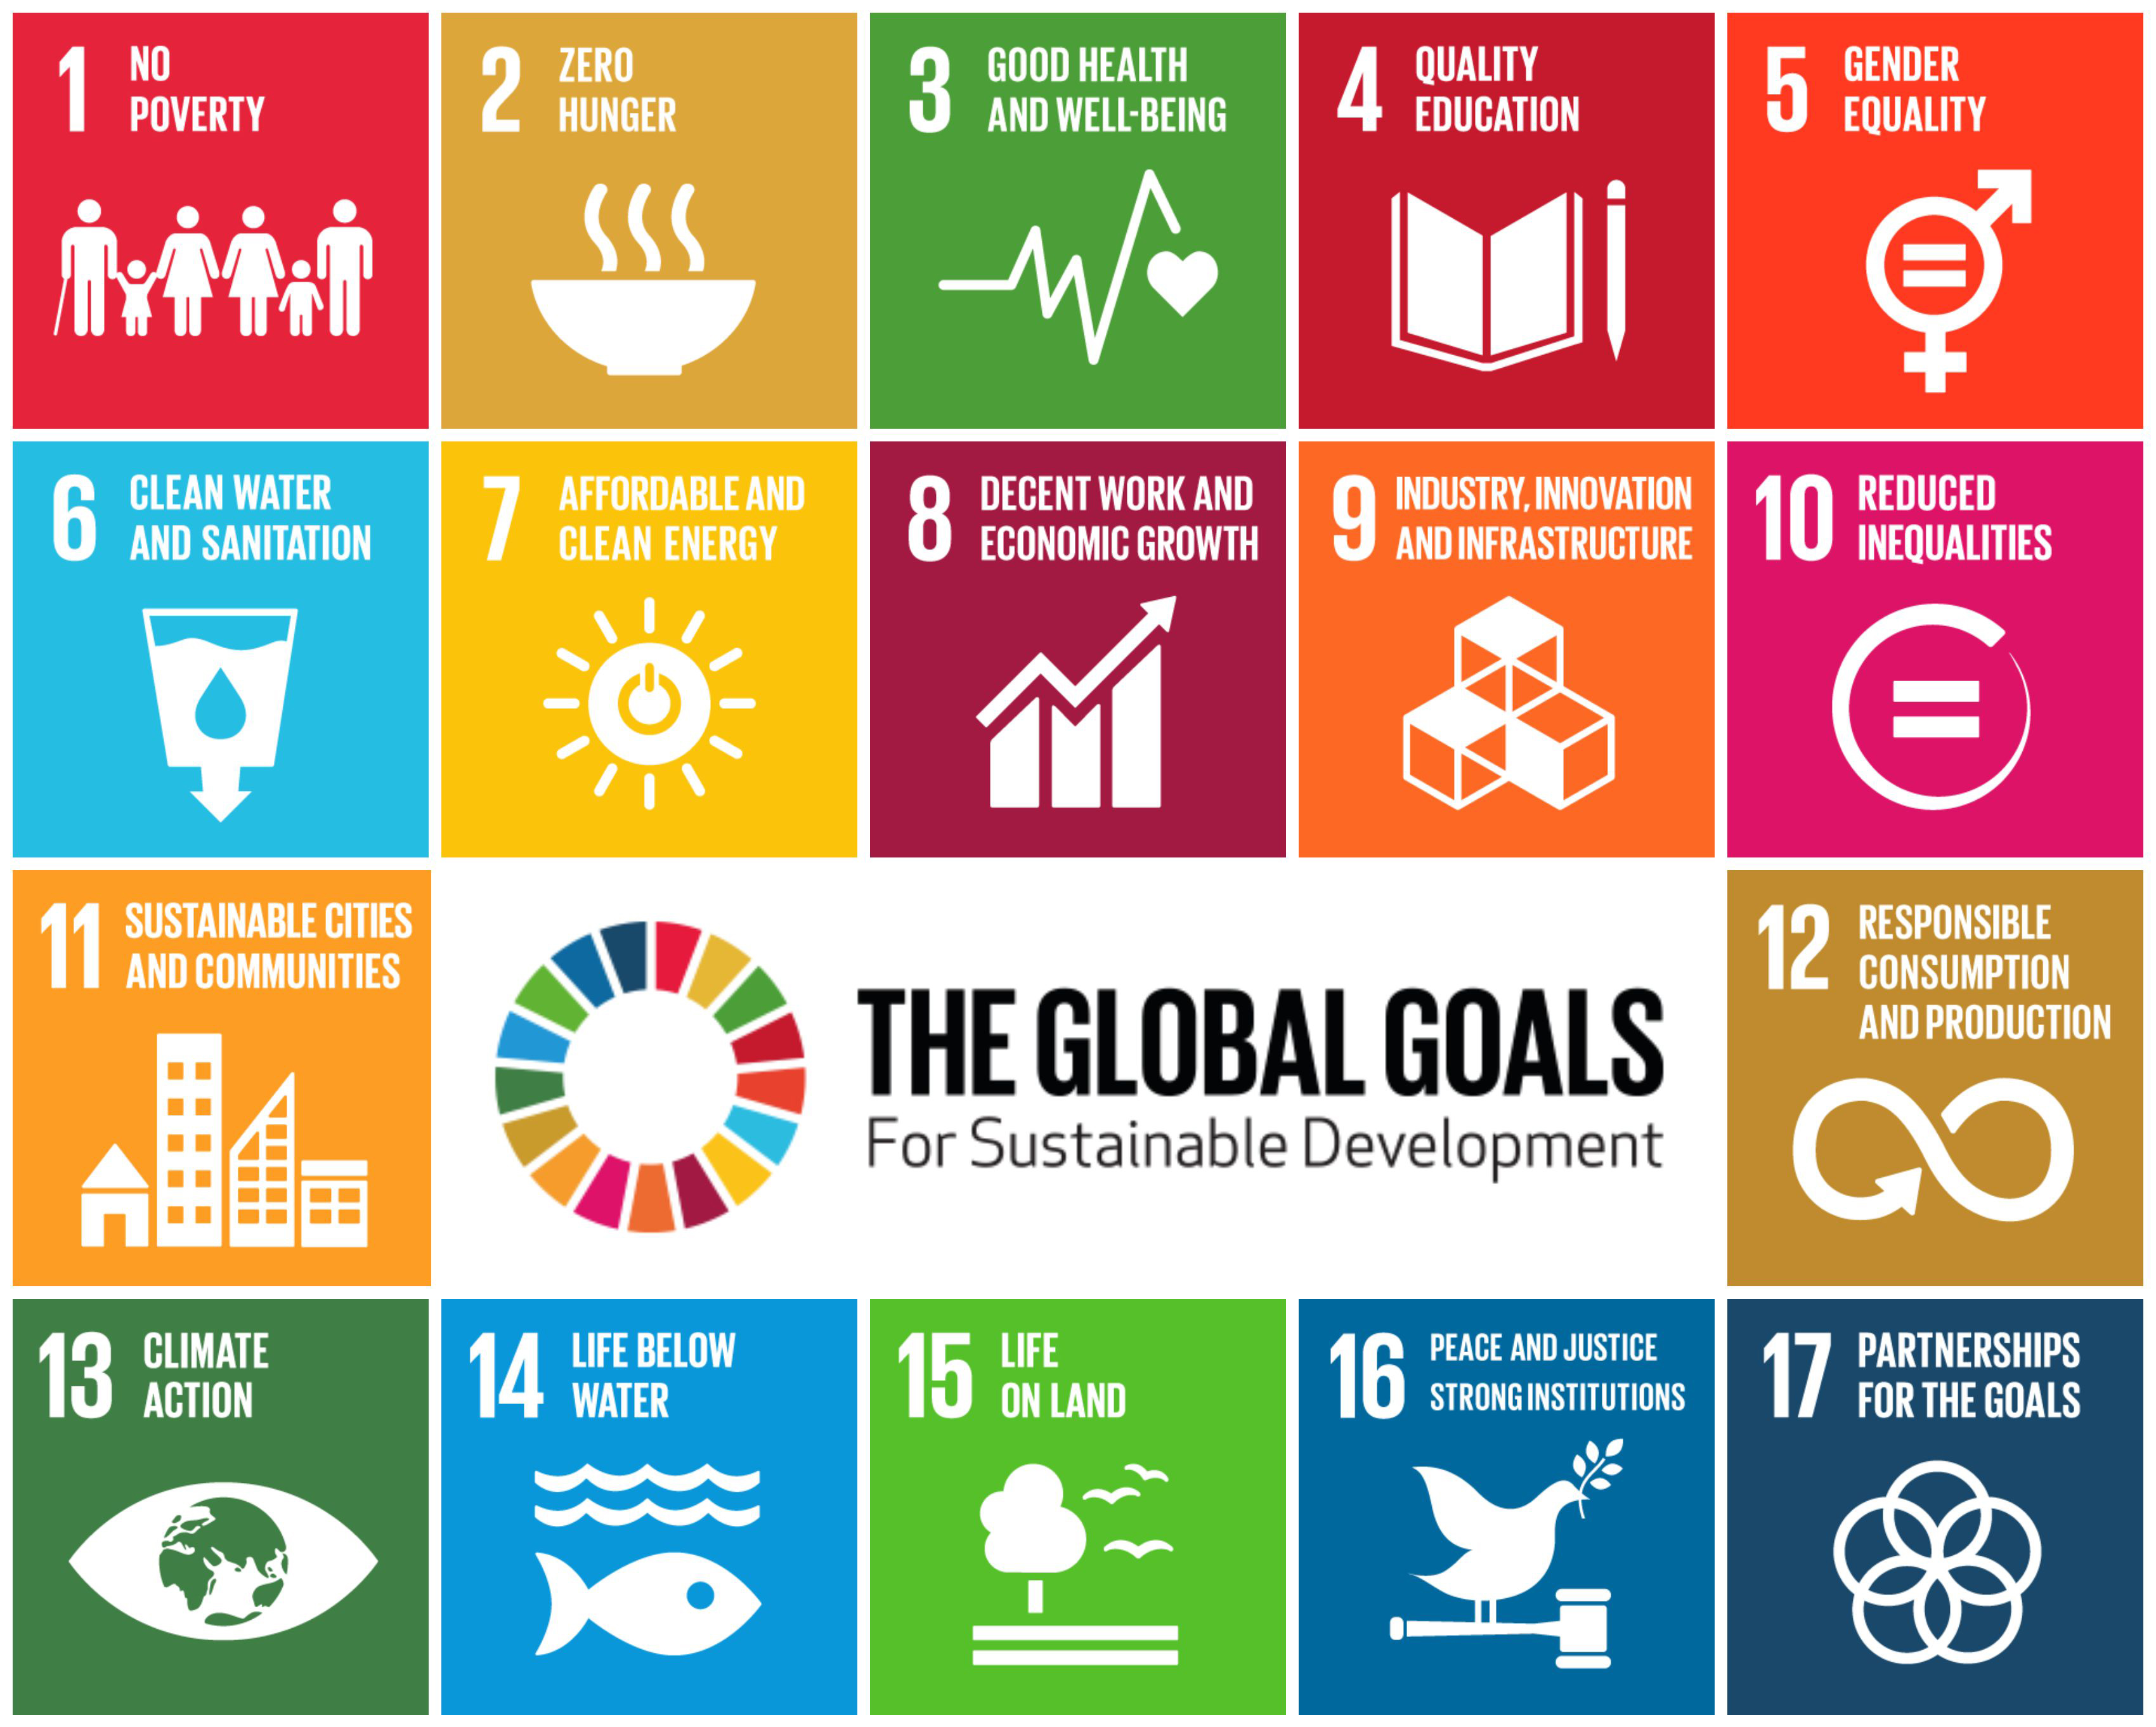
\includegraphics[width=0.7\textwidth]{goals}
	\caption{A diagram listing the 17 Sustainable Development Goals}
	\label{fig:ha}
\end{figure}

But there are also some trade-offs or even win-win Situations because some goals can’t be reached at the same time.
Its important to create a condition in which all people have physical, social and economics access to food.

But what do we mean by Sustainability because there are many different views as to what contains a sustainable food system, and what falls within the scope of the term 'sustainability’. When we look at it sustainability implies the use of resources at rates that do not exceed the capacity of the Earth to replace them. For food, a sustainable system might be encompassing a range of issues such as security of the supply of food, health, safety, affordability, quality, a strong food industry in terms of jobs and growth and, at the same time, environmental sustainability, in terms of issues such as climate change, biodiversity, water and soil quality.

Overall I think we are on the right way because we already learned we can’t just do whatever we want with our wold. By setting goals for the future we have a concrete goal that we can reach together.
\subsection{Global Perspective on Food Affairs }
Jens Soth gave us an insight into the global perspective on food affairs. He firstly showed us why the earth is «shrinking». Shrinking means that the population of the earth is growing and the available resources per capita are decreasing. The main problems which are leading to a shrinking world are soil loss and degradation. But also, that in the developing countries the demand is rising for food which needs more resources than traditional food. For example, chocolate, which is a luxury good. Also the diminishing availability of water and phosphorus are contributing to a shrinking world. These factors are leading to a higher pressure on arable land per capita.

\begin{figure}[H]	
	\centering
	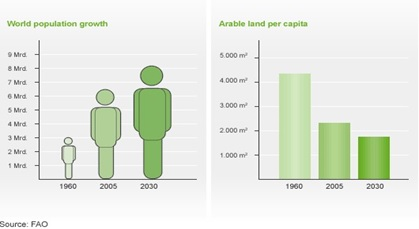
\includegraphics[width=0.7\textwidth]{muell}
	\caption{The world population is growing so that the arable land per capita  is decreasing.}
	\label{fig:ha}
\end{figure}
So we have to increase food production and sustainability at the same time. It is the wrong solution to just increase the use of fertilizers and pesticides. This solution is not good in the long-term. The solutions must take all factors into account the nature and all involved people to increase the production and be long-term sustainable meanwhile. A technical solution for agriculture which was explained by Jens Soth was the laser levelling of furrows and shorter furrows which conduce to 35\% less water use and 35\% more yield. 
What we learn is that the easy and short-term solutions are mostly the wrong ones, the solutions are complex and must be locally adapted and accepted by all involved people.
